%% need no \usepackage{Sweave.sty}
\documentclass[article]{jss}
\usepackage{amsmath}
\usepackage{amssymb}
\usepackage{amsthm}
\usepackage{graphicx}
\usepackage{natbib}
\usepackage{subfig}
\usepackage{todonotes}
\usepackage{multirow}

\author{Brenton Kenkel\\University of Rochester \And
  Curtis S. Signorino\\University of Rochester}
\Plainauthor{Brenton Kenkel, Curtis S. Signorino}

\title{Estimating Models of Strategic Interaction in \proglang{R}}
\Plaintitle{Estimating Models of Strategic Interaction in R}

\Abstract{
  Come up with this.
}

\Keywords{one, two, three}

\Address{
  Brenton Kenkel\\
  315A Harkness Hall\\
  Department of Political Science\\
  University of Rochester\\
  Rochester, NY 14627\\
  Email: \email{brenton.kenkel@gmail.com}
}

\begin{document}

\maketitle

\begin{Schunk}
\begin{Sinput}
R> options(useFancyQuotes = FALSE)
R> library("games")
R> packageVersion("games")
\end{Sinput}
\begin{Soutput}
[1] '1.0.0'
\end{Soutput}
\begin{Sinput}
R> data(leblang2003)
\end{Sinput}
\end{Schunk}

\section{Introduction}

\proglang{R} \citep{Rlang}

\section{Strategic statistical models}
\label{sec:models}

Strategic statistical models were first introduced to analyze international
crises and the outbreak of war \citep{Signorino1999}.  Signorino shows that
standard techniques like logistic regression are inappropriate when applied to
data generated by multi-agent strategic interactions, a point developed further
by \citet{Signorino2003a}.  He introduces a class of models that yield
consistent estimates of players' utilities when the structure of interaction is
known \citep[see also][]{Signorino2003}.  These models have since been applied
to data on U.S.\ congressional races \citep{Carson2003,Carson2005}, currency
markets \citep{Leblang2003}, armed deterrence \citep{Signorino2006},
international economic sanctions \citep{McLean2010}, territorial conflict
\citep{Carter2010a}, and Latin American governmental crises \citep{Helmke2010}.

Every strategic model is associated with a game form and solution concept.
First, the structure of the interaction must be known: the number of players,
the order in which they move, the number of actions each has available, and the
possible outcomes.  The purpose is to estimate players' utilities for each
outcome, usually as a function of covariates, from data on observed outcomes of
the game being played.  This requires the introduction of a stochastic
component, so that there is a non-degenerate probability distribution over
outcomes for any given set of coefficients (i.e., those on the covariates
describing players' utilities).  In particular, we will specify where error
enters the model and calculate the equilibrium outcome for each given set of
parameters and stochastic shocks, using the appropriate solution concept for the
assumed stochastic structure (see below).  The probability of each outcome can
then be obtained by assuming a distribution for the error terms.

The choice of stochastic structure is crucial for the estimation and
interpretation of utility parameters.  The \pkg{games} package implements
methods for two cases:
\begin{description}
  \item[Agent error] Each player's utility over outcomes is fixed and common
  knowledge.  However, there are perceptual errors that cause each player to
  choose the ``wrong'' action---i.e., not the one that maximizes her expected
  utility across the outcomes that are possible following each action.  This can
  be represented as a shock $\alpha_{mj}$ to Player $m$'s expected utility for
  taking action $j$, where the shock is realized immediately before $m$ makes
  her action choice (and hence is unknown to the preceding players).  We
  typically assume that each $\alpha_{mj}$ is drawn independently from a normal
  or logistic distribution.  The solution concept under agent error is quantal
  response equilibrium \citep{McKelvey1998}, wherein each player anticipates the
  probability of ``mistakes'' by the others and adjusts her expectations
  accordingly.

  \item[Private information] There is a different stochastic shock to each
  player's utility for each outcome.  We will write this as $\pi_{mk}$, for
  Player $m$ and outcome $k$.  The key assumption is that each player fully
  knows her utility for each outcome, but only knows the distribution of the
  shocks to the other players' outcome utilities.  The solution concept in this
  case is perfect Bayesian equilibrium: each player takes the action that gives
  her the highest expected utility, with respect to the realized shocks to her
  preferences and her expectations about the actions the other players will
  take.  Whereas the distribution over outcomes was induced by the possibility
  of wrong decisions in the agent error case, now it comes from the fact that
  observationally indistinguishable players may have different privately known
  preferences.  Except in the statistical ultimatum model, we will assume that
  each $\pi_{mk}$ is drawn from a normal distribution.
\end{description}
We illustrate both of these stochastic structures in the \code{egame12} example
below. \citet{Signorino2003} discusses these in greater depth, and concludes
from Monte Carlo experiments that models of the two types do not yield
appreciably different results when the underlying game form is relatively
simple.

\subsection[Illustration: The egame12 model]%
{Illustration: The \code{egame12} model}
\label{sec:egame12}

\begin{figure}[tp]
  \centering
  \subfloat[Agent error]%
  {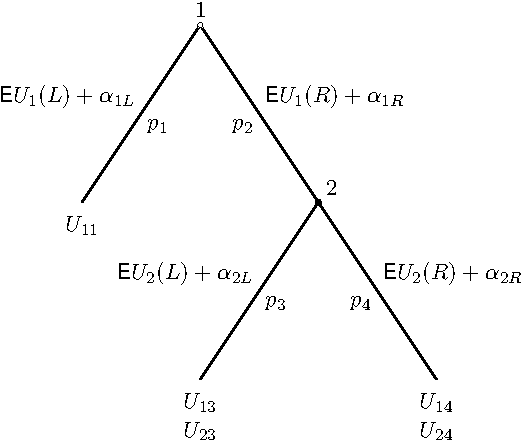
\includegraphics[width=0.55\textwidth]{img/egame12agent-crop}}
  
  \subfloat[Private information]%
  {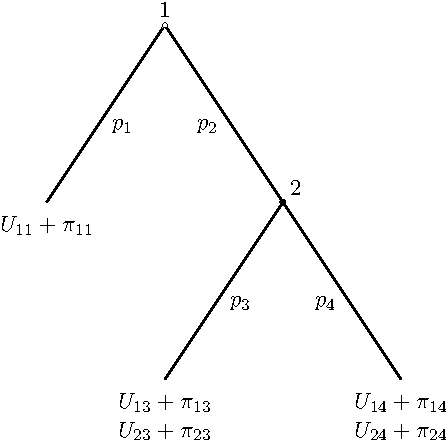
\includegraphics[width=0.5\textwidth]{img/egame12private-crop}}
  \caption{Game trees for the \code{egame12} model.}
  \label{fig:egame12-trees}
\end{figure}

The \code{egame12} model, with two players and three possible outcomes, is the
simplest strategic model.  The players are indexed $m = 1, 2$, and each has an
action set $a_m = \{L, R\}$.  The outcomes are indexed $Y = 1, 3, 4$.  The
structure of the interaction is as follows:
\todo[inline]{make game tree, refer}
\begin{enumerate}
  \item Player $1$ chooses his action $a_1$.  If $a_1 = L$, the game ends and
  the outcome is $Y = 1$.  Otherwise, if $a_1 = R$, Player 2 gets to move.
  \item Player $2$ chooses her action $a_2$.  If $a_2 = L$, the outcome is $Y =
  3$; if $a_2 = R$, the outcome is $Y = 4$.
\end{enumerate}
We use the following notation throughout the rest of the section:
\begin{center}
  \begin{tabular}{cl}
    notation & meaning \\ \hline
    $p_1$ & probability that $a_1 = L$ \\
    $p_2$ & probability that $a_1 = R$ \\
    $p_3$ & probability that $a_2 = L$, given $a_1 = R$ \\
    $p_4$ & probability that $a_2 = R$, given $a_1 = R$ \\
    $U_{mk}$ & systematic part of Player $m$'s utility from outcome $k$ \\
    $\E U_m(a)$ & $m$'s expected utility from taking action $a$
  \end{tabular}
\end{center}
\todo[inline]{need more words}

\todo[inline]{talk about betas, outcome probs, likelihood function}
\todo[inline]{u21 can't be estimated}
\todo[inline]{also mention egame122, egame123}

\begin{equation}
  \label{eq:log-lik}
  \log \ell(\beta \,|\, X, Y) = \sum_{Y_i = 1} \log p_{1i} + \sum_{Y_i = 3}
  (\log p_{2i} + \log p_{3i}) + \sum_{Y_i = 4} (\log p_{2i} + \log p_{4i})
\end{equation}

\subsubsection{Agent error}

Assume that each player receives a stochastic shock $\alpha_{mj}$ to her
expected utility for choosing $j \in \{L, R\}$, where each $\alpha_{mj}$ is
drawn independently from a normal distribution with mean $0$ and variance
$\sigma^2$.\footnote{The same calculations as follow can be applied in the case
  of errors with logistic distributions.}  To solve for the quantal response
equilibrium of the game, we will proceed via backward induction, solving for
Player $2$'s choice probabilities in order to find Player $1$'s.

If Player $2$'s turn is reached, her choice determines the outcome for sure.  We
thus have $\E U_2(L) = U_{23} = x_{23}^{\top} \beta_{23}$ and $\E U_2(R) =
U_{24} = x_{24}^{\top} \beta_{24}$.  The \textit{ex ante} probability that
Player $2$ chooses $R$ is
\begin{equation}
  \label{eq:p4-agent}
  \begin{aligned}
    p_4 &= \Prob[ \E U_2(R) + \alpha_{2R} \geq \E U_2(L) + \alpha_{2L}] \\
    &= \Prob [ \alpha_{2L} - \alpha_{2R} \leq x_{24}^{\top} \beta_{24} -
    x_{23}^{\top} \beta_{23} ] \\
    &= \Phi \left( \frac{x_{24}^{\top} \beta_{24} - x_{23}^{\top}
        \beta_{23}}{\sigma \sqrt{2}} \right),
  \end{aligned}
\end{equation}
where $\Phi(\cdot)$ is the standard normal CDF.  Since Player $2$ must choose
from $L$ or $R$, we have $p_3 = 1 - p_4$.  We now can solve for Player $1$'s
choice probabilities.  If Player $1$'s action is $L$, the outcome is $Y = 1$ for
certain.  However, if he chooses $R$, the outcome is a lottery over outcomes $3$
and $4$, with probabilities $p_3$ and $p_4$ respectively.  Since Player $1$ also
receives a shock to his expected utilities by action, his \textit{ex ante}
chance of choosing $R$ is
\begin{equation}
  \label{eq:p2-agent}
  \begin{aligned}
    p_2 &= \Prob[ \E U_1(R) + \alpha_{1R} \geq \E U_1(L) + \alpha_{1L}] \\
    &= \Prob [ \alpha_{1L} - \alpha_{1R} \leq p_3 x_{13}^{\top} \beta_{13} + p_4
    x_{14}^{\top} \beta_{14} - x_{11}^{\top} \beta_{11} ] \\
    &= \Phi \left(\frac{p_3 x_{13}^{\top} \beta_{13} + p_4 x_{14}^{\top}
        \beta_{14} - x_{11}^{\top} \beta_{11}}{\sigma \sqrt{2}} \right).
  \end{aligned}
\end{equation}
Because Player $1$ must choose $L$ or $R$, we have $p_1 = 1 - p_2$.  We can then
estimate the agent error model for a given dataset by substituting
\eqref{eq:p4-agent} and \eqref{eq:p2-agent} into the log-likehood function
\eqref{eq:log-lik}.

As in standard binary dependent variable models (e.g., GLMs with a logit or
probit link), the statistical model is not identified with respect to the scale
parameter $\sigma$, so it cannot be estimated \citep{Signorino1999,Lewis2003}.
The scale parameter is fixed to $\sigma = 1$ in all of the extensive-form models
in \pkg{games}, so each estimated utility coefficient $\hat{\beta}_{mkj}$ can be
interpreted as an estimate of the ratio $\beta_{mjk} / \sigma$.  Alternatively,
we allow for $\sigma$ to be modeled as a function of covariates, in which case
the regression coefficients for these variables can be estimated.  For details,
see the example in Section~\ref{sec:fitting}.

\subsubsection{Private information}

Assume there is an additive shock $\pi_{mk}$ to each outcome utility $U_{mk}$,
where each $\pi_{mk}$ is drawn independently from a normal distribution with
mean $0$ and variance $\sigma^2$.  We will again proceed by backward induction,
this time to solve for the perfect Bayesian equilibrium.

Player $2$ will choose $R$ if and only if $U_{24} + \pi_{24} \geq U_{23} +
\pi_{23}$.  The \textit{ex ante} probability of Player $2$ choosing $R$ is therefore
\begin{equation}
  \label{eq:p4-private}
  \begin{aligned}
    p_4 &= \Prob[ U_{24} + \pi_{24} \geq U_{23} + \pi_{23} ] \\
    &= \Prob[ \pi_{23} - \pi_{24} \leq x_{24}^{\top} \beta_{24} -  x_{23}^{\top}
    \beta_{23} ] \\
    &= \Phi \left(\frac{x_{24}^{\top} \beta_{24} -  x_{23}^{\top}
        \beta_{23}}{\sigma \sqrt{2}}\right).
  \end{aligned}
\end{equation}
As before, $p_3 = 1 - p_4$.  In addition, notice that \eqref{eq:p4-private} is
essentially the same as in \eqref{eq:p4-agent}, since Player $2$'s actions are
decisive over outcomes.  The same does not hold when we consider Player $1$'s
choice probabilities.  In particular, his expected utility for choosing $R$ in
the private-information case is
\begin{displaymath}
  \E U_1(R) = p_3 (x_{13}^{\top} \beta_{13} + \pi_{13}) + p_4 (x_{14}^{\top}
  \beta_{14} + \pi_{14})
\end{displaymath}
The \textit{ex ante} probability of Player $1$ selecting $R$ is
\begin{equation}
  \label{eq:p2-private}
  \begin{aligned}
    p_2 &= \Prob[ \E U_1(R) \geq \E U_1(L) ] \\
    &= \Prob[ p_3 (x_{13}^{\top} \beta_{13} + \pi_{13}) + p_4 (x_{14}^{\top}
    \beta_{14} + \pi_{14}) \geq x_{11}^{\top} \beta_{11} + \pi_{11}] \\
    &= \Prob[ \pi_{11} - p_3 \pi_{13} - p_4 \pi_{14} \leq p_3 x_{13}^{\top}
    \beta_{13} + p_4 x_{14}^{\top} \beta_{14} - x_{11}^{\top} \beta_{11} ] \\
    &= \Phi \left( \frac{p_3 x_{13}^{\top} \beta_{13} + p_4 x_{14}^{\top}
        \beta_{14} - x_{11}^{\top} \beta_{11}}{\sigma \sqrt{1 + p_3^2 + p_4^2}}
    \right).
  \end{aligned}
\end{equation}
In particular, the variance of Player $1$'s choice probabilities depends on
$p_3$ and $p_4$, which was not the case under agent error.  To estimate the
private information model, as before, substitute the choice probability
equations \eqref{eq:p4-private} and \eqref{eq:p2-private} into the
log-likelihood \eqref{eq:log-lik}.  As in the agent error model, the scale
parameter $\sigma$ cannot be estimated, so it is fixed to $1$ by the fitting
functions.

\subsection{The statistical ultimatum model}

\todo[inline]{go through the very basics}

\section{Specification and estimation}

\todo[inline]{introduce leblang as running example}

\subsection{Modeling player utilities}

The archetypal use of a strategic model is to estimate the effect of observed
factors on players' utility for each possible outcome\todo{citations}.  To avoid
an overabundance of parameters and potential inefficiency, analysts will
typically want to make some exclusion restrictions---i.e., to leave some
regressors out of some utility equations.\footnote{A necessary condition for
  identification in a strategic model is that no regressor, including the
  constant, appear in all of a player's utility equations for the outcomes
  reachable after her move \citep{Lewis2003}.  The fitting functions and
  \code{makeFormulas} enforce this condition.  One way to accomplish it is to
  fix each player's utility to $0$ for one outcome.  This comes without loss of
  generality, since Von Neumann--Morgenstern utilities are unique only up to an
  affine transformation \textbf{(cite)}.}  This necessitates the use of multiple
model formulas, which we handle via the \pkg{Formula} package
\citep{Formulapkg}.  The variables to include in each utility are specified
using the standard \code{formula} syntax, and each set is separated by a
vertical bar (\code{|}).  For example, in the \code{egame12} model, an analyst
may want to use the specification
\begin{align*}
  U_{11} &= \beta_{11,0} + \beta_{11,1} x_1 \\
  U_{13} &= 0 \\
  U_{14} &= \beta_{14,0} + \beta_{14,1} x_1 + \beta_{14,2} x_2 \\
  U_{24} &= \beta_{24,0} + \beta_{24,2} x_2,
\end{align*}
where $x_1$ and $x_2$ are observed variables.  The appropriate \code{Formula}
syntax is \code{y ~ x1 | 0 | x1 + x2 | x2}.

In some of the more complex models, such as \code{egame123} with its eight
utility equations, writing the model formulas manually may be daunting or prone
to error.  We provide two options for easing the process.  First, users may
specify the model formulas as a list; the fitting functions then use the
internal function \code{checkFormulas} to convert it to the appropriate
\code{Formula} object.
\begin{Schunk}
\begin{Sinput}
R> f1 <- list(u11 = y ~ x1, u13 = ~0, u14 = ~x1 + x2, u24 = ~x2)
R> games:::checkFormulas(f1)
\end{Sinput}
\begin{Soutput}
y ~ x1 | 0 | x1 + x2 | x2
<environment: 0x27d6ac0>
\end{Soutput}
\end{Schunk}
(Elements of the list need not be named; in fact, the names are ignored.)
Second, the function \code{makeFormulas} provides interactive prompts for
constructing the model formulas step by step.  The user only needs to supply the
name of the model he or she intends to fit and a character vector containing
outcome descriptions.  For the Leblang data, the appropriate call would look
like \code{makeFormulas(egame12, outcomes = c("no attack", "devaluation",
"defense"))}.  The following menu will appear at the \proglang{R} console:
\begin{Code}
Equation for player 1's utility from no attack: 

1: fix to 0
2: intercept only
3: regressors, no intercept
4: regressors with intercept

Selection: 
\end{Code}
If \code{3} or \code{4} is selected, the user will be prompted to enter a
space-separated list of variables to include in the utility equation of
interest.  We use functions from \pkg{stringr} \citep{stringrpkg} in parsing the
input.  The same menu will then be displayed for player 1's utility from
devaluation, player 1's utility from defense, and player 2's utility from
defense.  The final prompt will ask for the name of the variable (or variables;
see Section~\ref{sec:dep} below) containing information on the observed
outcomes.  The function will then return the \code{Formula} specification
corresponding to the given input, which can be supplied as the \code{formulas}
argument of the appropriate fitting function.

\subsection{Dependent variable specification}
\label{sec:dep}

For most of the models included in the \pkg{games} package, there are a few
different ways that the dependent variable might be stored in the dataset.  For
example, all of the following are plausible representations of the outcome
variable in the Leblang data:
\begin{itemize}
  \item Numeric indicators for the final outcome, where \code{1} means no
  currency attack, \code{2} means devaluation in response to an attack, and
  \code{3} means defense against an attack.
  \item Factor indicators for the final outcome, where the levels correspond to
  no attack, devaluation, and defense respectively.
  \item Binary variables representing each player's action.  The first would be
  coded \code{0} when there is no attack and \code{1} when there is an attack.
  The second would be coded \code{0} when the targeted country devalues and
  \code{1} when it defends the currency peg.
\end{itemize}
The \pkg{games} package allows for all of these types of specifications.  To use
a numeric or factor indicator for the final outcome, the form of the
specification is simply \code{y ~ .}, as in typical model formulas.  To use
binary indicators, the names of the indicators should be separated with \code{+}
signs on the left-hand side, as in \code{y1 + y2 ~ .}.  When using binary
indicators, unobserved outcomes---in this case, the value of \code{y2} when
\code{y1 == 0}---should \emph{not} be coded as \code{NA}s, as this will
typically result in their being removed from the dataset.

The method of specifying the dependent variable has no effect on the estimation
results, as shown in the next example.
\begin{Schunk}
\begin{Sinput}
R> leblang2003$attack <- as.numeric(leblang2003$outcome != "no attack")
R> leblang2003$defend <- as.numeric(leblang2003$outcome == "defense")
R> flb <- outcome ~ capcont + lreserves + overval + creditgrow + 
+     USinterest + service + contagion + prioratt - 1 | 1 | 1 | 
+     unifgov + lexports + preelec + postelec + rightgov + realinterest + 
+         capcont + lreserves
R> flb1 <- as.Formula(flb)
R> flb2 <- update(flb1, attack + defend ~ .)
R> leb1 <- egame12(flb1, data = leblang2003, link = "probit", type = "private")
R> leb2 <- egame12(flb2, data = leblang2003, link = "probit", type = "private")
\end{Sinput}
\end{Schunk}
\begin{Schunk}
\begin{Sinput}
R> all.equal(coef(leb1), coef(leb2), check.attributes = FALSE)
\end{Sinput}
\begin{Soutput}
[1] TRUE
\end{Soutput}
\end{Schunk}
The only difference is in the construction of the names of the utility
equations.  When binary action indicators are used, the outcome names are
inferred from the names of the action variables.  When numeric or factor outcome
variables are used, their values/levels are used as the outcome names.
\begin{Schunk}
\begin{Sinput}
R> cbind(leb1$equations, leb2$equations)
\end{Sinput}
\begin{Soutput}
     [,1]              [,2]                
[1,] "u1(no attack)"   "u1(~attack)"       
[2,] "u1(devaluation)" "u1(attack,~defend)"
[3,] "u1(defense)"     "u1(attack,defend)" 
[4,] "u2(defense)"     "u2(attack,defend)" 
\end{Soutput}
\end{Schunk}
The methods for specifying the dependent variable differ slightly
across models; see the help page of each fitting function for a list of
allowable specifications.

\subsection{Model fitting}
\label{sec:fitting}

Once the formula has been constructed, it is straightforward to fit a strategic
model.  All of the fitting functions contain the arguments \code{data},
\code{subset}, and \code{na.action}, which are used in the typical way to
construct the model frame.  In addition, the \code{method} argument is passed to
\code{maxLik} (from the \pkg{maxLik} package; \citealt{maxLikpkg}) to select an
optimization routine, and other parameters to control the process (e.g.,
\code{reltol}, \code{iterlim}) can be passed as named arguments.

Each fitting function returns an object inheriting from two S3 classes.  The
first is the \code{"game"} class, for which most of the methods of interest are
defined, including \code{print} and \code{summary}.  The second is the name of
the particular model that was fit; this is used by the \code{predict} methods.
For the most part, the elements of a \code{"game"} object are the same as those
of \code{"lm"} and \code{"glm"} objects (e.g., \code{coefficients},
\code{vcov}).  Pertinent differences include:
\begin{itemize}
  \item The \code{log.likelihood} element contains the vector of the $n$
  observationwise log-likelihoods evaluated at the parameter estimate, for use
  in non-nested model tests (see Section~\ref{sec:non-nest} below).
  \item The \code{y} element contains the outcome variable represented as a
  factor whose levels are the outcome names.
  \item The \code{link} and \code{type} elements store the link function and
  source of error respectively.
  \item The \code{equations} element contains the names of the utility equations
  and scale terms; this is used by \code{print.game} and \code{latexTable} to
  for grouping the parameters estimated.
\end{itemize}
Fitted \code{ultimatum} models contain some additional elements, which are
discussed below.

The nonparametric bootstrap is implemented as part of the fitting process via
the \code{boot} argument of the model functions.  To run the bootstrap on a
model that has already been estimated, use \code{update} as in the next example.
A status bar is printed by default, but it can be suppressed by setting
\code{bootreport = FALSE}.
\begin{Schunk}
\begin{Sinput}
R> set.seed(42)
R> leb1 <- update(leb1, boot = 100)
\end{Sinput}
\end{Schunk}
% doing this manually b/c no printing from cached blocks
\begin{Code}
Running bootstrap iterations...
=================================================================
\end{Code}
Bootstrap results are stored in the \code{boot.matrix} element of the fitted
model object.  When a model has been bootstrapped, the default behavior of
\code{summary.game} is to use the bootstrap results to calculate standard error
estimates.
\begin{Schunk}
\begin{Sinput}
R> summary(leb1)
\end{Sinput}
\begin{Soutput}
Call:
egame12(formulas = flb1, data = leblang2003, link = "probit", 
    type = "private", boot = 100)

Coefficients:
                            Estimate Std. Error z value Pr(>|z|)
u1(no attack):capcont        -0.4525     0.3352   -1.35  0.17710
u1(no attack):lreserves       0.2292     0.0629    3.64  0.00027
u1(no attack):overval        -0.4413     0.1400   -3.15  0.00162
u1(no attack):creditgrow     -0.0648     0.0380   -1.71  0.08800
u1(no attack):USinterest     -0.0505     0.0507   -1.00  0.31902
u1(no attack):service        -0.0288     0.0401   -0.72  0.47291
u1(no attack):contagion      -0.1159     0.0435   -2.66  0.00773
u1(no attack):prioratt       -0.1218     0.0457   -2.66  0.00771
u1(devaluation):(Intercept)  -3.6648     0.3855   -9.51  < 2e-16
u1(defense):(Intercept)      -3.1385     0.4057   -7.74  1.0e-14
u2(defense):(Intercept)       0.4269     1.7442    0.24  0.80663
u2(defense):unifgov          -0.3568     0.3862   -0.92  0.35559
u2(defense):lexports         -0.1997     0.1891   -1.06  0.29085
u2(defense):preelec           1.6632     1.9215    0.87  0.38672
u2(defense):postelec          1.0623     0.9031    1.18  0.23947
u2(defense):rightgov         -0.9358     0.5176   -1.81  0.07058
u2(defense):realinterest      1.7955     1.0693    1.68  0.09312
u2(defense):capcont           0.0656     1.7098    0.04  0.96940
u2(defense):lreserves         0.3099     0.2046    1.51  0.12985

Standard errors estimated from bootstrap results

Log-likelihood: -482.02
AIC: 1002.0
No. observations: 7240 
\end{Soutput}
\end{Schunk}
To see the normal-theory standard errors instead, supply the option
\code{useboot = FALSE} to the \code{summary} call.

The other arguments for the fitting functions depend on whether the model is one
of the discrete extensive form games or the statistical ultimatum game.

\subsubsection{Extensive-form models}

The stochastic structure of the extensive-form models is specified via the
arguments \code{link} and \code{type}.  The \code{link} argument is used to
specify the distributional form of the error terms: \code{"probit"} for normal,
\code{"logit"} for type I extreme value.  The \code{type} argument specifies
whether the source of randomness is \code{"agent"} error or \code{"private"}
information.  Normal errors must be used in the case of private information; if
a model is specified with \code{link = "logit"} and \code{type = "private"}, a
warning will be issued and a probit link will be enforced.

The error variance $\sigma$ normally is not estimable on its own, as noted above
in Section~\ref{sec:models}.  This is no longer the case if $\sigma$ is modeled
as function of known covariates:
\begin{displaymath}
  \sigma = \exp(\gamma_1 Z_1 + \gamma_2 Z_2 + \ldots + \gamma_k Z_k).
\end{displaymath}
The argument \code{sdformula} is used to estimate $\gamma$ for such a model.
The formula should be one-sided, with nothing to the left of the \code{~}, as in
the following example with the Leblang data.
\begin{Schunk}
\begin{Sinput}
R> leb3 <- egame12(outcome ~ lreserves + overval - 1 | 1 | 1 | preelec + 
+     realinterest, sdformula = ~prioratt - 1, data = leblang2003, 
+     link = "probit", type = "private")
\end{Sinput}
\end{Schunk}
\begin{Schunk}
\begin{Sinput}
R> summary(leb3)
\end{Sinput}
\begin{Soutput}
Call:
egame12(formulas = outcome ~ lreserves + overval - 1 | 1 | 1 | 
    preelec + realinterest, data = leblang2003, link = "probit", 
    type = "private", sdformula = ~prioratt - 1)

Coefficients:
                            Estimate Std. Error z value Pr(>|z|)
u1(no attack):lreserves       0.2264     0.0464    4.88  1.1e-06
u1(no attack):overval        -0.4381     0.0836   -5.24  1.6e-07
u1(devaluation):(Intercept)  -3.0137     0.2470  -12.20  < 2e-16
u1(defense):(Intercept)      -2.8410     0.2275  -12.49  < 2e-16
u2(defense):(Intercept)      -0.0190     0.1988   -0.10   0.9239
u2(defense):preelec           1.3690     0.6402    2.14   0.0325
u2(defense):realinterest      1.4943     0.5610    2.66   0.0077
log(sigma):prioratt           0.0427     0.0186    2.29   0.0221

Standard errors estimated from inverse Hessian

Log-likelihood: -495.37
AIC: 1006.7
No. observations: 7240 
\end{Soutput}
\end{Schunk}
\todo[inline]{interpret results, mention log(sigma) vs log(lambda), talk about
  separate errors by player}

The extensive-form models also allow for estimation of the error variance when
the average payoffs are known to the analyst, such as in data from lab
experiments.  In this case, the payoffs can be specified with the
\code{fixedUtils} argument.  The only information needed from the model formula
is the outcome variable, so the \code{formulas} argument can be written in the
form \code{y ~ .} or \code{y ~ 1}.  When the argument \code{fixedUtils} is used,
the default behavior is to estimate a single common scale parameter, as in the
next example.
\begin{Schunk}
\begin{Sinput}
R> lebfixed <- egame12(outcome ~ ., data = leblang2003, fixedUtils = c(1, 
+     -1, 0, 1), link = "probit", type = "private")
\end{Sinput}
\end{Schunk}
\begin{Schunk}
\begin{Sinput}
R> summary(lebfixed)
\end{Sinput}
\begin{Soutput}
Call:
egame12(formulas = outcome ~ ., data = leblang2003, link = "probit", 
    type = "private", fixedUtils = c(1, -1, 0, 1))

Coefficients:
           Estimate Std. Error z value Pr(>|z|)
log(sigma)  -1.0513     0.0199   -52.9   <2e-16

Standard errors estimated from inverse Hessian

Fixed terms:
  u1(no attack) u1(devaluation)     u1(defense)     u2(defense) 
              1              -1               0               1 

Log-likelihood: -646.54
AIC: 1295.1
No. observations: 7240 
\end{Soutput}
\end{Schunk}
As before, \code{sdByPlayer} can be used to estimate a separate scale parameter
for each player, and \code{sdformulas} to specify the scale term(s) as a
function of covariates.

\subsubsection[The ultimatum model]{The \code{ultimatum} model}

In the ultimatum model, each observation consists of the value of the offer made
by Player 1 and whether Player 2 accepted it.  By assumption, there is an
exogenous upper bound on the size of the offer, which is specified via
\code{maxOffer}.  The lower bound is always 0.  It is important to be able to
identify which offers were at one of these boundary points, since the
log-likelihood of an observation depends on whether the offer was interior.  If
offers are stored as floating-point numbers, naive equality tests may
misclassify some boundary observations as interior.  To mitigate this, we use
the argument \code{offertol} and code an offer $x$ as meeting the lower bound if
$x < \mbox{\code{offertol}}$ and the upper bound if $x > \mbox{\code{maxOffer}}
- \mbox{\code{offertol}}$.  Unless there are extremely slight differences
between observed offers, on the order of $1 \times 10^{-8}$, the default value
of \code{offertol} should suffice for most analyses.

The arguments \code{s1} and \code{s2} are for fixing the scale parameters of the
stochastic component of the players' reservation values.  If either of these is
left unspecified, it is estimated.  We recommend fixing \code{s2}, since
attempts to estimate it often run into numerical stability issues
\citep{Ramsay2009}.

The model formula for \code{ultimatum} should be written in the form \code{offer
  + accept ~ R1 | R2}, where \code{R1} and \code{R2} contain the variables for
Player 1's and 2's reservation values respectivelyx.  Some researchers may only
have access to data on offer size, but not whether the offer was accepted.  For
such datasets, run \code{ultimatum} with the argument \code{outcome = "offer"}
and specify the model formula as \code{offer ~ R1 | R2}.  Parameters for Player
2's reservation value are still estimable in this case, since the optimal offer
for Player 1 depends on his or her expectations of the probability of
acceptance.  Even when acceptance data are available, the option \code{outcome =
  "offer"} may be useful for making formal comparisons of the statistical
ultimatum model to OLS or GLS models of offer size, as in \citet{Ramsay2009}.
For more on model comparison, see Section~\ref{sec:non-nest} below.

\todo[inline]{example}

\begin{Schunk}
\begin{Sinput}
R> load("ultimatum2010.rda")
\end{Sinput}
\end{Schunk}
\begin{Schunk}
\begin{Sinput}
R> ult1 <- ultimatum(offer + accept ~ gender1 | gender2, maxOffer = 100, 
+     data = ultimatum2010, s2 = 3)
\end{Sinput}
\end{Schunk}
\begin{Schunk}
\begin{Sinput}
R> print(ult1)
\end{Sinput}
\begin{Soutput}
A fitted strategic model

CALL:

ultimatum(formulas = offer + accept ~ gender1 | gender2, data = ultimatum2010, 
    maxOffer = 100, s2 = 3)

COEFFICIENTS:

  Player 1's reservation value:
                        
     (Intercept)  62.198
     gender1     -25.409

  Player 2's reservation value:
                         
     (Intercept) 37.68430
     gender2     -0.89703

  Logged scale parameter for player 1:
                        
     estimated as 3.9341

  Logged scale parameter for player 2:
                    
     fixed to 1.0986
\end{Soutput}
\end{Schunk}


\subsection{Convergence}

The log-likelihood functions for strategic models are not globally concave, so
convergence to a global maximum is not guaranteed.  We provide two means for
averting convergence problems.  First, in all of the \code{egame} models, the
default starting values come from statistical backward induction (SBI), a
two-step method that uses ordinary probit or logistic regression models to
obtain consistent estimates of the parameters \citep{Bas2007}.\footnote{SBI is
  based on the assumption of agent error, so the estimates technically are not
  consistent for private-information models.  However, for strategic models of
  relatively low complexity like those available in the \pkg{games} package, the
  assumption of agent error or private information makes little difference to
  the parameter estimates \citep{Signorino2003}.}

\todo[inline]{finish talking about sbi, mention sqrt(2) correction}

\begin{Schunk}
\begin{Sinput}
R> data(student_offers)
R> stu1 <- ultimatum(offer + accept ~ gender1 | gender2, data = student_offers, 
+     maxOffer = 100, s2 = 1)
R> profstu1 <- profile(stu1, which = 1:3)
\end{Sinput}
\end{Schunk}
% must include manually since Sweave doesn't print errors
\begin{Code}  
Warning message:
In profile.game(stu1, which = 1:3) :
  some profiled fits have higher log-likelihood than original fit;
  refit the model using "profile" option
\end{Code}

\begin{figure}[t]
  \centering
\includegraphics{games-plotprof}
\caption{Output of \code{plot.profile}.}
\label{fig:plot-profile}
\end{figure}

\begin{Schunk}
\begin{Sinput}
R> plot(profstu1)
\end{Sinput}
\end{Schunk}

\subsection{Reporting results}
\label{sec:report}

\begin{table}[p]
%% latex table generated in R 2.12.2 by games package
%% Wed Mar 23 10:19:28 2011
%% remember to include \usepackage{multirow} in your preamble

\begin{table}[htbp]
\begin{center}
\begin{tabular}{lcccc}
\hline
 & u1(no attack) & u1(devaluation) & u1(defense) & u2(defense) \\
\hline
\multirow{2}{*}{(Intercept)} & \multirow{2}{*}{} & $-$3.6648 & $-$3.1385 & 0.4269 \\
 &  & (0.3855) & (0.4057) & (1.7442) \\[2pt]
\multirow{2}{*}{capcont} & $-$0.4525 & \multirow{2}{*}{} & \multirow{2}{*}{} & 0.0656 \\
 & (0.3352) &  &  & (1.7098) \\[2pt]
\multirow{2}{*}{lreserves} & 0.2292 & \multirow{2}{*}{} & \multirow{2}{*}{} & 0.3099 \\
 & (0.0629) &  &  & (0.2046) \\[2pt]
\multirow{2}{*}{overval} & $-$0.4413 & \multirow{2}{*}{} & \multirow{2}{*}{} & \multirow{2}{*}{} \\
 & (0.1400) &  &  &  \\[2pt]
\multirow{2}{*}{creditgrow} & $-$0.0648 & \multirow{2}{*}{} & \multirow{2}{*}{} & \multirow{2}{*}{} \\
 & (0.0380) &  &  &  \\[2pt]
\multirow{2}{*}{USinterest} & $-$0.0505 & \multirow{2}{*}{} & \multirow{2}{*}{} & \multirow{2}{*}{} \\
 & (0.0507) &  &  &  \\[2pt]
\multirow{2}{*}{service} & $-$0.0288 & \multirow{2}{*}{} & \multirow{2}{*}{} & \multirow{2}{*}{} \\
 & (0.0401) &  &  &  \\[2pt]
\multirow{2}{*}{contagion} & $-$0.1159 & \multirow{2}{*}{} & \multirow{2}{*}{} & \multirow{2}{*}{} \\
 & (0.0435) &  &  &  \\[2pt]
\multirow{2}{*}{prioratt} & $-$0.1218 & \multirow{2}{*}{} & \multirow{2}{*}{} & \multirow{2}{*}{} \\
 & (0.0457) &  &  &  \\[2pt]
\multirow{2}{*}{unifgov} & \multirow{2}{*}{} & \multirow{2}{*}{} & \multirow{2}{*}{} & $-$0.3568 \\
 &  &  &  & (0.3862) \\[2pt]
\multirow{2}{*}{lexports} & \multirow{2}{*}{} & \multirow{2}{*}{} & \multirow{2}{*}{} & $-$0.1997 \\
 &  &  &  & (0.1891) \\[2pt]
\multirow{2}{*}{preelec} & \multirow{2}{*}{} & \multirow{2}{*}{} & \multirow{2}{*}{} & 1.6632 \\
 &  &  &  & (1.9215) \\[2pt]
\multirow{2}{*}{postelec} & \multirow{2}{*}{} & \multirow{2}{*}{} & \multirow{2}{*}{} & 1.0623 \\
 &  &  &  & (0.9031) \\[2pt]
\multirow{2}{*}{rightgov} & \multirow{2}{*}{} & \multirow{2}{*}{} & \multirow{2}{*}{} & $-$0.9358 \\
 &  &  &  & (0.5176) \\[2pt]
\multirow{2}{*}{realinterest} & \multirow{2}{*}{} & \multirow{2}{*}{} & \multirow{2}{*}{} & 1.7955 \\
 &  &  &  & (1.0693) \\[2pt]
\hline \hline
Log-likelihood & $-$482.0155 \\
 $N$ & 7240\\
\hline
\end{tabular}
\end{center}
\end{table}\caption{Replication of \citeauthor{Leblang2003}'s \citeyearpar{Leblang2003}
  results.}
\label{tab:leb1}
\end{table}

\section{Analyzing fitted models}

\subsection{Predicted probabilities}
\label{sec:pred-prob}

\subsection{Non-nested model comparisons}
\label{sec:non-nest}


\section*{Acknowledgments}

We thank the Wallis Institute for Political Economy at the University of
Rochester for financial support.


\bibliography{games,software}

\end{document}
